% فصل ۶ (فارسی، مستقل): روش‌های حل و نتایج شبیه‌سازی
% کامپایل:  xelatex chapter6_fa.tex   (دو بار برای ارجاع‌ها)
% شکل‌ها: ./figures/   فونت‌ها: ./fonts/
% موارد علامت‌گذاری شده با TODO پس از پایان اجرای کامل یادگیری تقویتی به‌روزرسانی شوند.
\documentclass[12pt,oneside]{report}
\usepackage[a4paper,margin=2.5cm]{geometry}
\usepackage{amsmath,amssymb}
\usepackage{graphicx}
\usepackage{booktabs}
\usepackage{float}
\usepackage{enumitem}
\usepackage[hidelinks]{hyperref}
\usepackage{xepersian}
\settextfont[Path=fonts/, Scale=1.15, BoldFont={IRNazaninBold.ttf}, ItalicFont={IRNazaninIranic.ttf}]{IRNazanin.ttf}
\setlist{itemsep=2pt}
\setcounter{chapter}{5}
\linespread{1.3}

\newcommand{\cU}{\mathcal{U}}
\newcommand{\cB}{\mathcal{B}}
\newcommand{\cN}{\mathcal{N}}

\begin{document}

\chapter{روش‌های حل و نتایج شبیه‌سازی}\label{ch:results}

در این فصل مسئله‌ی تخصیص مشترک منابع رادیویی و محاسباتی شبکه‌ی \lr{O-RAN} به دو روش حل و نتایج آن‌ها مقایسه می‌شود:
\begin{enumerate}
	\item روش مبتنی بر بهینه‌سازی (محدب و ترکیبیاتی) که جواب بهینه را همراه با یک کران پایین تضمین‌شده ارائه می‌دهد و مرجع مقایسه است؛
	\item روش‌های یادگیری تقویتی عمیق دو مقیاس زمانی شامل یادگیری چندعاملی با دو عامل \lr{TD3} (\lr{MARL})، روش ترکیبی یک عامل یادگیری تقویتی (\lr{TD3} یا \lr{SAC}) به همراه بهینه‌سازی محدب، و یک عامل واحد \lr{SAC}.
\end{enumerate}
بخش \ref{sec:setup} شبکه و مسئله را تعریف می‌کند، بخش‌های \ref{sec:opt} و \ref{sec:rl} دو خانواده‌ی روش حل را شرح می‌دهند و بخش‌های \ref{sec:res_opt} تا \ref{sec:res_rl} نتایج را ارائه می‌کنند.

% =====================================================================================
\section{مدل شبکه و مسئله}\label{sec:setup}

\subsection{شبکه و ترافیک}
شبکه شامل $B=4$ واحد رادیویی (\lr{RU}) روی یک شبکه‌ی منظم در ناحیه‌ای به ابعاد $1000\times1000$ متر، $|\cN^e|=4$ گره لبه و $|\cN^r|=2$ گره منطقه‌ای \lr{O-Cloud} است.
هر واحد رادیویی $M=25$ بلوک منبع (\lr{PRB}) با پهنای باند کل ۲۵ مگاهرتز و توان بیشینه‌ی ۴۰ \lr{dBm} دارد.
بهره‌ی کانال کاربر $u$ روی بلوک $m$ واحد $b$ برابر $G_{b,u}h_{b,u,m}$ است که در آن تضعیف مسیر با نمای ۳ و محوشدگی رایلی مدل شده است؛ توان نویز ۱۷۴- \lr{dBm/Hz} است و تداخل بین واحدهای رادیویی صفر فرض شده است.
کاربران به طور یکنواخت توزیع شده و به طور متوازن بین سه برش جدول \ref{tab:slices} تقسیم می‌شوند.
مقیاس زمانی کوچک یک برش زمانی ۱ میلی‌ثانیه‌ای و مقیاس زمانی بزرگ $K=10$ برش زمانی است. برای هر $U\in\{5,10,15,20\}$ نتایج میانگین پنج چیدمان تصادفی است.

\begin{table}[H]
	\centering
	\caption{پارامترهای برش‌ها}\label{tab:slices}
	\begin{latin}
		\begin{tabular}{lccccc}
			\toprule
			Slice & $D_s^{QoS}$ & packet size $q$ & arrival rate $\lambda$ & weight $\delta_s$ & speed \\
			\midrule
			eMBB  & 25\,ms   & 1500\,B & 100\,pkt/s & 0.5 & 1.5\,m/s \\
			URLLC & 5\,ms    & 200\,B  & 50\,pkt/s  & 0.9 & 1.5\,m/s \\
			mMTC  & 1000\,ms & 20\,B   & 1\,pkt/s   & 0.1 & static \\
			\bottomrule
		\end{tabular}
	\end{latin}
\end{table}

\paragraph{پردازش و انتقال.}
واحد مرکزی (\lr{CU}) و واحد توزیع‌شده (\lr{DU}) هر واحد رادیویی روی گره‌های \lr{O-Cloud} جاگذاری می‌شوند. گره لبه یک هسته‌ی $3.4$ گیگاهرتز و گره منطقه‌ای ده هسته دارد.
پردازش هر ۱ مگابیت بر ثانیه در \lr{CU} به $0.00175\times3.4$ و در \lr{DU} به $0.04\times3.4$ گیگاهرتز نیاز دارد و هزینه‌ی هر چرخه‌ی پردازنده در لبه ده برابر گره منطقه‌ای است.
لینک‌های \lr{fronthaul} (\lr{RU}--\lr{DU}) و \lr{midhaul} (\lr{DU}--\lr{CU}) به ترتیب ۱۰ و ۱ برابر نرخ داده‌ی کاربران را روی فیبر ۱۰۰ و ۱۰ گیگابیت بر ثانیه حمل می‌کنند.

\paragraph{سه تصمیم مدل‌سازی.}
\begin{itemize}
	\item \textbf{واحد اندازه‌ی بسته بایت است.} با برداشت «کیلوبیت»، بار ترافیکی از ظرفیت لینک‌ها فراتر رفته و همه‌ی جاگذاری‌ها ناممکن می‌شوند.
	\item \textbf{هر گره \lr{O-Cloud} یک صف $M/M/c$ است} ($c$ = تعداد هسته‌ها) که زمان انتظار آن با فرمول \lr{Erlang-C} و زمان سرویس هر بسته با $\tilde c^{\,l}q_u/f_{\text{core}}$ محاسبه می‌شود؛ به این ترتیب تأخیر پردازش به محل جاگذاری وابسته می‌شود. بودجه‌ی تأخیر \lr{fronthaul} برابر ۱۰۰ میکروثانیه است.
	\item \textbf{قید زمان‌بندی:} اگر \lr{CU} و \lr{DU} یک واحد رادیویی روی گره‌های مختلف باشند، مجموع تأخیر انتشار \lr{CU}$\to$\lr{DU}، پردازش \lr{CU} و ارسال \lr{midhaul} نباید از $\theta=1$ میلی‌ثانیه بیشتر شود.
\end{itemize}

\subsection{متغیرهای تصمیم و تأخیر}
متغیرهای تصمیم عبارت‌اند از: اتصال کاربر $\alpha_u^b\in\{0,1\}$، تخصیص بلوک $\kappa_u^{b,m}\in\{0,1\}$، توان بلوک $\omega_u^{b,m}\ge0$ و جاگذاری $\psi_b^{l,n}\in\{0,1\}$ تابع $l\in\{\mathrm{CU},\mathrm{DU}\}$ واحد $b$ روی گره $n$.
نرخ کاربر $u$ برابر است با
\begin{equation}\label{eq:rate}
	R_u=\sum_{b}\alpha_u^b\sum_{m}\kappa_u^{b,m}\,B_p\log_2\!\Big(1+\frac{\omega_u^{b,m}G_{b,u}h_{b,u,m}}{N_0B_p}\Big),
\end{equation}
که $B_p$ پهنای باند هر بلوک است. تأخیر انتها به انتهای کاربر $u$ متصل به واحد $b$ برابر است با
\begin{equation}\label{eq:e2e}
	D_u^{e2e}=\underbrace{\frac{1}{R_u/q_u-\lambda_u}}_{\text{\rl{صف رادیویی}}}
	+\underbrace{D_b^{\text{proc}}}_{\text{\rl{صف گره‌ها}}}
	+\underbrace{D_b^{\text{tr}}}_{\text{\rl{ارسال}}}
	+\underbrace{D_b^{\text{prop}}}_{\text{\rl{انتشار}}} .
\end{equation}
هزینه‌ی $\bar\phi$ میانگین هزینه‌ی پردازنده‌ی گره‌های میزبان توابع است.

\subsection{مسئله‌ی بهینه‌سازی}
چون تأخیر و هزینه مقیاس‌های بسیار متفاوتی دارند، هر دو جمله بی‌بعد شده‌اند:
\begin{equation}\label{eq:J}
	J=\sum_{s=1}^{3}\Big(\delta_s\,\frac{1}{|\cU_s|}\sum_{u\in\cU_s}\frac{D_u^{e2e}}{D_s^{QoS}}+(1-\delta_s)\frac{\bar\phi}{\phi_{\max}}\Big),\qquad \phi_{\max}=2\max_n\phi_n .
\end{equation}
در این تابع مقدار ۱ برای جمله‌ی تأخیر یعنی رسیدن به بودجه‌ی \lr{QoS} برش. معادل آن $J=\sum_uw_uD_u^{e2e}+K\bar\phi$ با $w_u=\delta_s/(|\cU_s|D_s^{QoS})$ است. مسئله عبارت است از
\begin{equation}\label{eq:problem}
	\min_{\alpha,\kappa,\omega,\psi}\ J
	\quad\text{s.t.}\quad
	\begin{cases}
		\sum_b\alpha_u^b=1, \quad \kappa_u^{b,m}\le\alpha_u^b, \quad \sum_u\kappa_u^{b,m}\le1 & \text{\rl{(اتصال، بلوک)}}\\
		\sum_{u,m}\kappa_u^{b,m}\omega_u^{b,m}\le P_b^{\max} & \text{\rl{(توان)}}\\
		\sum_n\psi_b^{l,n}=1,\quad \text{\rl{ظرفیت پردازش و لینک}} & \text{\rl{(جاگذاری)}}\\
		\text{\rl{پایداری همه‌ی صف‌ها}},\ D_u^{e2e}\le D_s^{QoS} & \text{\rl{(کیفیت سرویس)}}\\
		\text{\rl{بودجه‌ی fronthaul و قید زمان‌بندی}}\ \theta & \text{\rl{(زمان‌بندی)}}
	\end{cases}
\end{equation}
که یک مسئله‌ی برنامه‌ریزی عدد صحیح مختلط غیرخطی (\lr{MINLP}) است.

% =====================================================================================
\section{حل مبتنی بر بهینه‌سازی}\label{sec:opt}

\paragraph{تجزیه‌ی دقیق.}
بدون تداخل، نرخ هر کاربر فقط به بلوک‌ها و توان واحد رادیویی خودش بستگی دارد. بنابراین با ثابت بودن اتصال $\alpha$، تابع هدف به صورت دقیق تجزیه می‌شود:
\begin{equation}\label{eq:decomp}
	J=\sum_{b\in\cB}V_b\big(\kappa_b,\omega_b;\alpha,\sigma_b\big)+I(\psi;\alpha).
\end{equation}
در این رابطه:
\begin{itemize}
	\item $V_b$ جمله‌های وابسته به نرخ واحد $b$ است: صف رادیویی و تأخیر ارسال \lr{fronthaul}/\lr{midhaul}.
	\item $V_b$ از جاگذاری فقط از طریق $\sigma_b=\mathbf{1}[\text{\rl{CU و DU واحد $b$ جدا باشند}}]$ اثر می‌پذیرد.
	\item $I$ جمله‌های مستقل از نرخ است: انتشار، صف گره‌ها و هزینه.
\end{itemize}
پس برای هر اتصال کافی است دو مسئله‌ی رادیویی برای هر واحد ($\sigma_b=0,1$) حل شود و سپس جاگذاری روی مقادیر ذخیره‌شده بهینه گردد. حل‌کننده چهار لایه دارد.

\paragraph{۱- تخصیص توان (محدب، بهینه‌ی سراسری).}
با تخصیص بلوک ثابت، $R_u$ نسبت به توان مقعر و $1/(R_u/q_u-\lambda_u)$ نسبت به $R_u$ محدب و نزولی است؛ پس $V_b$ نسبت به $\omega$ محدب است. هر تکرار سه گام دارد:
\begin{enumerate}
	\item $V_b$ نسبت به نرخ‌ها خطی‌سازی می‌شود (وزن‌های $\kappa_u=-\partial V_b/\partial R_u>0$).
	\item مسئله‌ی بیشینه‌سازی نرخ وزن‌دار با پرکردن آب به صورت دقیق حل می‌شود:
	\begin{equation}\label{eq:wf}
		p_m=\Big[\frac{\kappa_{o(m)}B_p}{\mu\ln2}-\frac{1}{a_m}\Big]^+,\qquad \sum_mp_m=P_b^{\max},
	\end{equation}
	که در آن $o(m)$ صاحب بلوک $m$، $a_m$ نسبت بهره به نویز آن و $\mu$ قیمت توان است و به صورت بسته روی بلوک‌های مرتب‌شده محاسبه می‌شود.
	\item یک جستجوی خطی دقیق به سمت این نقطه انجام می‌شود.
\end{enumerate}
نقطه‌ی ثابت این روند شرایط \lr{KKT} را برآورده می‌کند و بنابراین بهینه‌ی سراسری است؛ در آزمون‌ها همواره برابر یا بهتر از حل‌کننده‌ی \lr{Clarabel} (از طریق \lr{CVXPY}) بوده است.

\paragraph{۲- تخصیص بلوک‌های منبع (ترکیبیاتی).}
برای واحدهای کوچک همه‌ی تخصیص‌ها شمرده می‌شوند. در غیر این صورت حل‌کننده سه گام انجام می‌دهد:
\begin{enumerate}
	\item یک تخصیص حریصانه بر اساس بهبود حاشیه‌ای می‌سازد؛
	\item آن را با جابه‌جایی تک بلوک بهبود می‌دهد؛
	\item در مرحله‌ی پالایش، ۱۲ حرکت برتر (جابه‌جایی یک بلوک یا تعویض دو بلوک بین کاربران) را با توان بهینه‌ی دقیق ارزیابی می‌کند و بهترین بهبود واقعی را می‌پذیرد تا هیچ حرکتی بهبود ندهد.
\end{enumerate}
هر کاربر متصل حداقل یک بلوک می‌گیرد، وگرنه صف رادیویی آن ناپایدار است.

\paragraph{۳- جاگذاری \lr{CU}/\lr{DU} (شمارش کامل).}
با $\alpha$ ثابت و مقادیر ذخیره‌شده‌ی $V_b(\sigma_b)$، هر جاگذاری فقط با محاسبات جبری ارزیابی می‌شود. همه‌ی $N^{2B}=6^8=1\,679\,616$ جاگذاری به صورت برداری در چند ثانیه شمرده می‌شوند و همه‌ی قیود پردازش، لینک، پایداری صف و زمان‌بندی بررسی می‌شوند؛ پس جاگذاری برای هر اتصال دقیقاً بهینه است.

\paragraph{۴- اتصال کاربران (جستجوی محلی چندشروعی).}
فضای اتصال $B^U$ است ($4^{20}\approx10^{12}$ برای $U=20$). جستجو از ۸ نقطه‌ی شروع (اتصال به بهترین کانال و ترکیب‌های تصادفی از ۲ یا ۳ واحد برتر هر کاربر) آغاز می‌شود. در هر گام یک کاربر به یکی از سه واحد برتر خود منتقل می‌شود و حرکت در صورت کاهش $J$ (با جاگذاری بهینه‌شده) پذیرفته می‌شود. بهترین جواب در پایان پالایش و جاگذاری آن دوباره با شمارش کامل بهینه می‌شود.

\paragraph{کران پایین تضمین‌شده.}
با آزادسازی بلوک‌ها و اتصال به مقادیر کسری و استفاده از نرخ پرسپکتیو $x\,B_p\log_2(1+a\,s/x)$ یک مسئله‌ی محدب به دست می‌آید. دوگان لاگرانژی آن برای هر سه‌تایی (واحد، بلوک، کاربر) فرم بسته دارد و طبق دوگانی ضعیف به ازای هر ضرایب، یک کران پایین معتبر است؛ ضرایب با \lr{L-BFGS} روی یک تقریب نرم (که خود کران معتبر است) بیشینه می‌شوند. دو فاصله گزارش می‌شود:
\begin{itemize}
	\item \textbf{فاصله‌ی شرطی:} روی همه‌ی انتخاب‌های بلوک، توان و جاگذاری به ازای اتصال یافته‌شده؛
	\item \textbf{فاصله‌ی سراسری:} با آزادسازی اتصال؛ این کران با افزایش $U$ سست می‌شود و حد بالای محافظه‌کارانه‌ی فاصله‌ی واقعی است.
\end{itemize}

\paragraph{صحت‌سنجی.}
روی ۱۲ نمونه‌ی کوچک ($B=N=2$، $U=M=3$) که همه‌ی متغیرها قابل شمارش هستند، روش مقیاس‌پذیر در \textbf{۱۲ از ۱۲} نمونه دقیقاً به بهینه‌ی سراسری رسید. در آزمون‌های واحد نیز تجزیه‌ی \eqref{eq:decomp} با محاسبه‌ی مستقیم شاخص‌ها مطابقت دارد.

% =====================================================================================
\section{یادگیری تقویتی دو مقیاس زمانی}\label{sec:rl}
مسئله به صورت یک فرایند تصمیم‌گیری مارکوف دو مقیاس زمانی مدل می‌شود: در هر برش زمانی بلوک‌ها و توان $(\kappa,\omega)$ و در هر $K=10$ برش اتصال و جاگذاری $(\alpha,\psi)$ تعیین می‌شود. هر اپیزود ۱۰ گام بزرگ (۱۰۰ برش) است. در هر اپیزود آموزشی چیدمان کاربران از نو تولید می‌شود ولی شبکه ثابت است. سیاست آموخته‌شده بدون نویز کاوش روی همان نمونه‌ای ارزیابی می‌شود که جواب بهینه برای آن محاسبه شده است.

\paragraph{حالت (\lr{State}).}
حالت مقیاس بزرگ برابر است با
\begin{equation}\label{eq:sL}
	s^L_t=\Big[\tfrac{1}{40}\big(10\log_{10}G_{b,u}+120\big),\ \mathbf e^{\text{slice}}_u,\ \mathbf e^{\alpha}_u,\ \mathbf e^{\mathrm{CU}}_b,\ \mathbf e^{\mathrm{DU}}_b,\ \rho_n,\ \phi_n/\phi_{\max}\Big].
\end{equation}
اجزای این بردار عبارت‌اند از:
\begin{itemize}
	\item بهره‌ی مقیاس بزرگ نرمال‌شده‌ی همه‌ی زوج‌های (واحد، کاربر)؛
	\item بردارهای \lr{one-hot} برش و واحد فعلی هر کاربر؛
	\item بردارهای \lr{one-hot} گره فعلی \lr{CU} و \lr{DU} هر واحد؛
	\item بهره‌وری پردازنده $\rho_n$ و هزینه‌ی هر گره.
\end{itemize}
حالت مقیاس کوچک علاوه بر آن، محوشدگی هر کاربر روی همه‌ی بلوک‌های واحد خدمت‌دهنده را دارد: $s^S_t=[s^L_t,\ 10\log_{10}h_{b(u),u,m}/10]$. برای $U=10$ ابعاد حالت $170$ و $420$ و برای $U=20$ برابر $280$ و $780$ است.

\paragraph{عمل (\lr{Action}) و نگاشت آن.}
عمل‌ها پیوسته و در $[-1,1]$ هستند و طوری نگاشت می‌شوند که قیود اتصال، انحصار بلوک، توان و جاگذاری همواره برقرار باشند:
\begin{itemize}
	\item \textbf{عمل بزرگ} $a^L\in[-1,1]^{UB+2BN}$ (۸۸ بعد برای $U=10$): یک امتیاز برای هر زوج (کاربر، واحد) و برای هر زوج (واحد، گره) جداگانه برای \lr{CU} و \lr{DU}. تصمیم با بیشینه‌ی امتیاز به اضافه‌ی یک پیشین باقیمانده گرفته می‌شود:
	\begin{equation}\label{eq:decL}
		b(u)=\arg\max_b\big(a^L_{u,b}+\beta\,\mathbf{1}[b=b^{\text{st}}(u)]\big),\qquad
		n^l(b)=\arg\max_n\big(a^L_{l,b,n}+\beta\,\mathbf{1}[n=n^{l,\text{st}}(b)]\big),
	\end{equation}
	که $(b^{\text{st}},n^{\text{st}})$ بهترین تصمیم ثابت است (اتصال به بهترین کانال و بهترین سناریوی ثابت جاگذاری). پس عمل صفر دقیقاً سیاست مرجع ثابت را تولید می‌کند و عامل فقط انحراف سودمند را یاد می‌گیرد.
	\item \textbf{عمل کوچک} $a^S=[z,y]\in[-1,1]^{2U}$: برای کاربران هر واحد:
	\begin{itemize}
		\item سهم بلوک $\pi_u=\mathrm{softmax}(\tau z)_u$ و سهم توان $\varpi_u=\mathrm{softmax}(\tau y)_u$ است؛
		\item تعداد بلوک‌ها با روش بزرگ‌ترین باقیمانده تعیین می‌شود (حداقل یک بلوک برای هر کاربر)؛
		\item بلوک‌ها به ترتیب کیفیت کانال بین کاربران تقسیم می‌شوند؛
		\item توان هر کاربر به طور مساوی روی بلوک‌هایش پخش می‌شود و واحد همیشه از تمام توان $P_b^{\max}$ استفاده می‌کند.
	\end{itemize}
\end{itemize}

\paragraph{پاداش (\lr{Reward}).}
پاداش مشترک همه‌ی عامل‌ها برابر است با
\begin{equation}\label{eq:reward}
	r_t=-\min\Big\{\frac{J_t+\varrho\,N^{\text{viol}}_t\,J_{\text{ref}}}{J_{\text{ref}}},\ r_{\max}\Big\}-c_a\,\overline{a_t^{2}},
\end{equation}
که در آن:
\begin{itemize}
	\item $J_t$ تابع هدف \eqref{eq:J} است؛
	\item $N^{\text{viol}}_t$ تعداد قیود نقض‌شده است (ظرفیت، پایداری صف، \lr{QoS}، بودجه‌ی \lr{fronthaul}، زمان‌بندی)؛
	\item $J_{\text{ref}}$ مقدار هدف بهترین سناریوی ثابت برای چیدمان فعلی است؛
	\item $\varrho=1$ و $r_{\max}=10$ است؛
	\item $\overline{a_t^2}$ میانگین مربع عمل‌های اعمال‌شده است.
\end{itemize}
با این مقیاس، سیاست ثابت پاداش حدود $-1$ و جواب بهینه پاداش $-J^*/J_{\text{ref}}>-1$ می‌گیرد. پاداش عامل بزرگ میانگین $K$ برش دوره‌ی آن است (انتقال نیمه‌مارکوف). اپیزودها فقط به دلیل محدودیت زمانی پایان می‌یابند، پس انتقال‌ها غیرپایانی ذخیره می‌شوند.

\paragraph{روش‌های مقایسه‌شده.}
\begin{itemize}
	\item \textbf{\lr{MARL} (دو عامل \lr{TD3}):} یک عامل \lr{TD3} برای هر مقیاس زمانی؛ منتقد عامل کوچک عمل جاری عامل بزرگ را نیز می‌بیند (آموزش متمرکز، اجرای غیرمتمرکز).
	\item \textbf{روش ترکیبی (\lr{TD3} یا \lr{SAC} + بهینه‌سازی محدب):} عامل فقط اتصال و جاگذاری را تعیین می‌کند و در هر برش، بلوک‌ها با جستجوی محلی و توان با \eqref{eq:wf} (۴۰ تکرار) بهینه می‌شوند.
	\item \textbf{عامل واحد \lr{SAC}:} یک عامل در هر برش $[a^L,a^S]$ را تولید می‌کند و $a^L$ فقط در ابتدای هر دوره‌ی $K$ برشی اعمال می‌شود.
\end{itemize}

\begin{table}[H]
	\centering
	\caption{پارامترهای یادگیری تقویتی}\label{tab:rl}
	\begin{latin}
		\begin{tabular}{p{8.5cm}p{5.5cm}}
			\toprule
			Parameter & Value \\
			\midrule
			Actor / critic hidden layers (small agent) & (1024, 512) / (512, 256) \\
			Actor / critic learning rate & $10^{-4}$ / $10^{-3}$ \\
			Discount $\gamma$, soft update $\tau_{\text{soft}}$ & 0.99, 0.005 \\
			Replay buffer; batch (small / large agent) & 50\,000; 128 / 64 \\
			Random warm-up transitions (small / large) & 500 / 50 \\
			TD3 exploration / target noise, clip, policy delay & 0.1 / 0.2, 0.5, 2 \\
			SAC initial temperature (auto-tuned) & 0.2 \\
			Residual prior $\beta$; share factor $\tau$; action penalty $c_a$ & 1; 1; 0.1 \quad (TODO: confirm) \\
			Large agent: layers, gradient steps per transition & (1024, 512), 10 \quad (TODO: confirm) \\
			Episodes $\times$ slots & 1000 $\times$ 100 \\
			\bottomrule
		\end{tabular}
	\end{latin}
\end{table}

% =====================================================================================
\section{نتایج: جواب بهینه در برابر سناریوهای ثابت}\label{sec:res_opt}
جدول \ref{tab:p5} و شکل \ref{fig:p5} جواب بهینه را با این روش‌های مرجع مقایسه می‌کنند:
\begin{itemize}
	\item سه سناریوی ثابت جاگذاری: همه در لبه؛ \lr{CU} منطقه‌ای و \lr{DU} لبه؛ همه منطقه‌ای؛
	\item بهترین این سه برای هر چیدمان (بهترین ثابت)؛
	\item جستجوی جاگذاری: بهینه‌سازی جاگذاری با اتصال ثابت به بهترین کانال.
\end{itemize}

\begin{table}[H]
	\centering
	\caption{تابع هدف نرمال‌شده $J$ (میانگین ۵ چیدمان)؛ بهبود نسبت به بهترین سناریوی ثابت}\label{tab:p5}
	\begin{latin}
		\resizebox{\textwidth}{!}{%
		\begin{tabular}{ccccccccc}
			\toprule
			$U$ & all edge & CU reg./DU edge & best static & placement search & \textbf{optimum} & gain & cond.\ gap & global gap \\
			\midrule
			5  & 0.1806 & 0.1186 & 0.0561 & 0.0355 & \textbf{0.0310} & 33.2\% & 0.001\% & 4.5\% \\
			10 & 0.3416 & 0.2032 & 0.0432 & 0.0413 & \textbf{0.0344} & 19.5\% & 0.35\%  & 7.1\% \\
			15 & 0.4305 & 0.2502 & 0.0487 & 0.0479 & \textbf{0.0384} & 20.8\% & 1.51\%  & 10.0\% \\
			20 & 0.5923 & 0.3350 & 0.0525 & 0.0520 & \textbf{0.0426} & 18.5\% & 0.26\%  & 11.3\% \\
			\bottomrule
		\end{tabular}}
	\end{latin}
\end{table}

\begin{figure}[H]
	\centering
	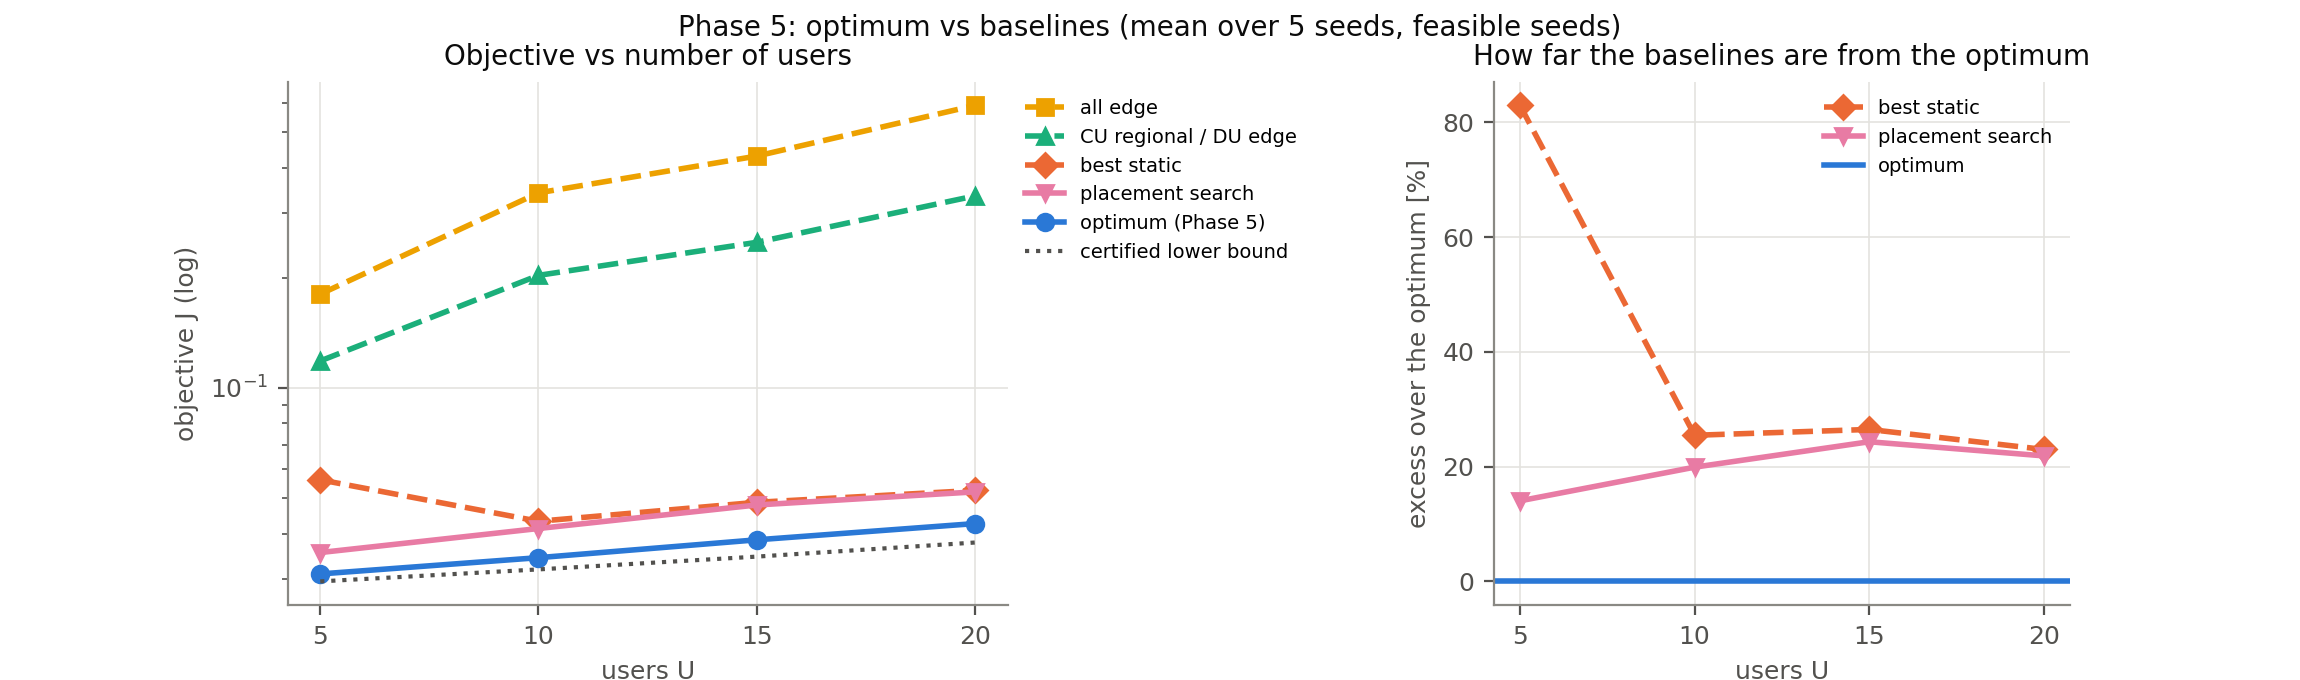
\includegraphics[width=\textwidth]{figures/phase5_optimum_vs_baselines.png}
	\caption{چپ: تابع هدف جواب بهینه، روش‌های مرجع و کران پایین تضمین‌شده بر حسب تعداد کاربران. راست: فاصله‌ی روش‌های مرجع از جواب بهینه}\label{fig:p5}
\end{figure}

\begin{itemize}
	\item \textbf{جواب بهینه در همه‌ی چیدمان‌ها از بهترین سناریوی ثابت بهتر است} و بهبود میانگین $18.5$ تا $33.2$ درصد است. عدد $U=5$ تحت تأثیر یک چیدمان است که در آن سناریوی «همه منطقه‌ای» قید ظرفیت را نقض می‌کند و بهترین سناریوی ثابت قابل قبول، سناریوی بسیار ضعیف‌تری است؛ بدون این چیدمان بهبود حدود ۱۲ درصد است.
	\item \textbf{بهینه‌سازی جاگذاری به تنهایی فقط بخش کوچکی از این بهبود را به دست می‌آورد} (۱۴ تا ۲۴ درصد بالاتر از بهینه)؛ بهینه‌سازی مشترک اتصال، بلوک، توان و جاگذاری ضروری است.
	\item \textbf{سناریوهای «همه در لبه» ۴ تا ۱۴ برابر بدترند}: تک هسته‌ی لبه صف پردازشی طولانی می‌سازد و هر چرخه‌ی پردازنده در لبه ده برابر گران‌تر است.
	\item \textbf{فاصله‌ی شرطی کمتر از $0.4$ درصد است} (در $U=15$ برابر $1.5$ درصد): به ازای اتصال یافته‌شده، بلوک، توان و جاگذاری عملاً بهینه‌اند. فاصله‌ی سراسری ($4.5$ تا $11.3$ درصد) به دلیل سست شدن کران اتصال رشد می‌کند و فاصله‌ی واقعی را بیش از حد نشان می‌دهد.
	\item \textbf{زمان حل سریع رشد می‌کند}: حدود ۶ دقیقه برای $U=5$، ۴۷ دقیقه برای $U=10$ و چند ساعت برای $U\ge15$. این زمان برای تصمیم‌گیری در هر برش زمانی بسیار زیاد است و انگیزه‌ی استفاده از یادگیری تقویتی است.
\end{itemize}

% =====================================================================================
\section{نتایج: موجودیت‌های مدل سیستم در جواب بهینه}\label{sec:res_ent}
در این بخش نمونه‌ی $U=20$ (چیدمان ۰) با جزئیات بررسی می‌شود.

\paragraph{اتصال کاربران و جاگذاری.}
شکل \ref{fig:assoc} نشان می‌دهد که اتصال لزوماً به قوی‌ترین واحد نیست: ۶ کاربر از ۲۰ کاربر (از هر برش ۲ کاربر) به واحد دیگری متصل شده‌اند. کاربران پرترافیک \lr{eMBB} و \lr{URLLC} بین واحدها متوازن شده‌اند (۲ تا ۵ کاربر در هر واحد) و ۶ کاربر \lr{mMTC} با بار ناچیز روی \lr{RU4} جمع شده‌اند.
در این نمونه \lr{CU} و \lr{DU} هر واحد در یک گره منطقه‌ای قرار گرفته‌اند: ده هسته صف پردازشی را کوتاه و ارزان نگه می‌دارد و جداسازی تأخیر \lr{midhaul} اضافه می‌کند.
در کل چیدمان‌ها، جداسازی \lr{CU} و \lr{DU} برای $U\le10$ هرگز و برای $U\ge15$ در ۲۵ تا ۵۰ درصد واحدها انتخاب شده است. سهم توابع لبه با افزایش بار از ۶۵ درصد ($U=5$) به ۳۵ درصد ($U=20$) کاهش می‌یابد.

\begin{figure}[H]
	\centering
	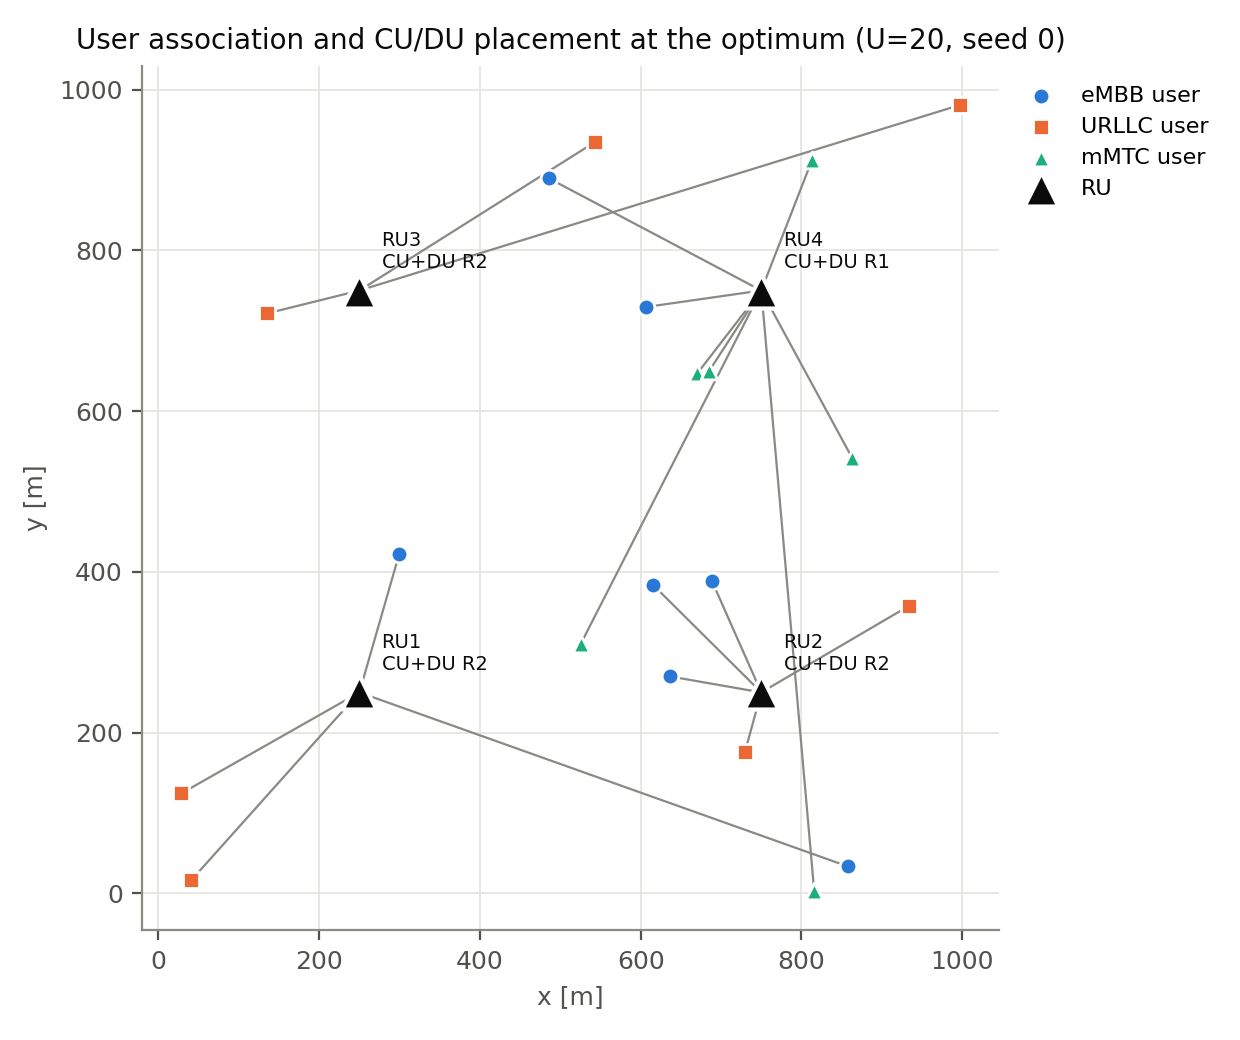
\includegraphics[width=0.78\textwidth]{figures/system_association.png}
	\caption{اتصال کاربران و جاگذاری \lr{CU}/\lr{DU} در جواب بهینه ($U=20$)}\label{fig:assoc}
\end{figure}

\paragraph{توان و بلوک‌های منبع.}
شکل \ref{fig:power} نکات زیر را نشان می‌دهد:
\begin{itemize}
	\item کاربران \lr{eMBB} و \lr{URLLC} هر کدام ۵ تا ۱۰ بلوک و ۱ تا ۶ وات دریافت می‌کنند؛
	\item هر کاربر \lr{mMTC} فقط یک بلوک با حدود $0.03$ وات می‌گیرد که برای پایداری صف آن کافی است؛
	\item در هر واحد، توزیع توان از قاعده‌ی پرکردن آب \eqref{eq:wf} پیروی می‌کند: بلوک‌های ضعیف‌تر توان کمتری می‌گیرند یا به کاربران کم‌بار داده می‌شوند.
\end{itemize}

\begin{figure}[H]
	\centering
	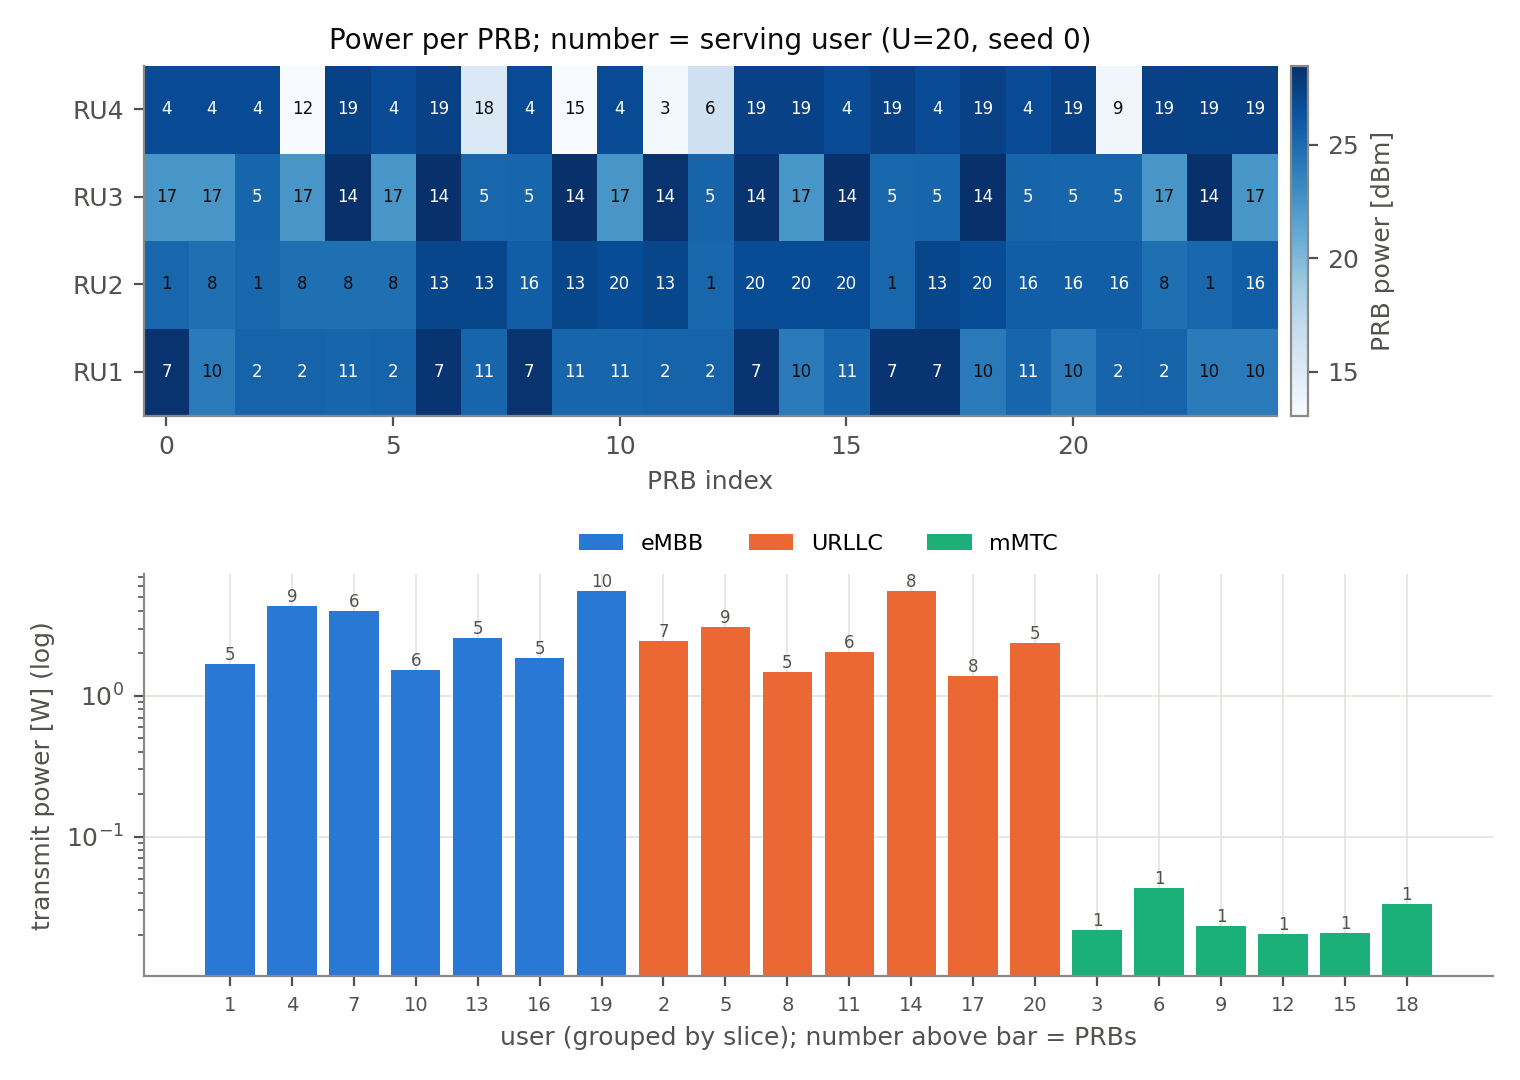
\includegraphics[width=0.9\textwidth]{figures/system_power.png}
	\caption{بالا: توان هر بلوک (عدد = کاربر خدمت‌گیرنده). پایین: توان کل و تعداد بلوک هر کاربر به تفکیک برش}\label{fig:power}
\end{figure}

\paragraph{تأخیر.}
شکل \ref{fig:delay} تأخیر انتها به انتهای هر کاربر را به اجزای آن تفکیک می‌کند:
\begin{itemize}
	\item \textbf{\lr{eMBB}:} پردازش غالب است (حدود ۷۰ درصد)، زیرا بسته‌های ۱۵۰۰ بایتی چرخه‌های پردازشی زیادی لازم دارند.
	\item \textbf{\lr{URLLC}:} پردازش بزرگ‌ترین جزء است (حدود ۵۵ درصد) و پس از آن صف رادیویی و انتشار قرار دارند.
	\item \textbf{\lr{mMTC}:} انتشار غالب است.
	\item \textbf{\lr{QoS}:} همه‌ی کاربران با فاصله‌ی زیاد زیر بودجه‌ی خود هستند: بیشینه $0.87$ میلی‌ثانیه در برابر ۲۵ برای \lr{eMBB} و حدود $0.13$ در برابر ۵ میلی‌ثانیه برای \lr{URLLC}.
\end{itemize}

\begin{figure}[H]
	\centering
	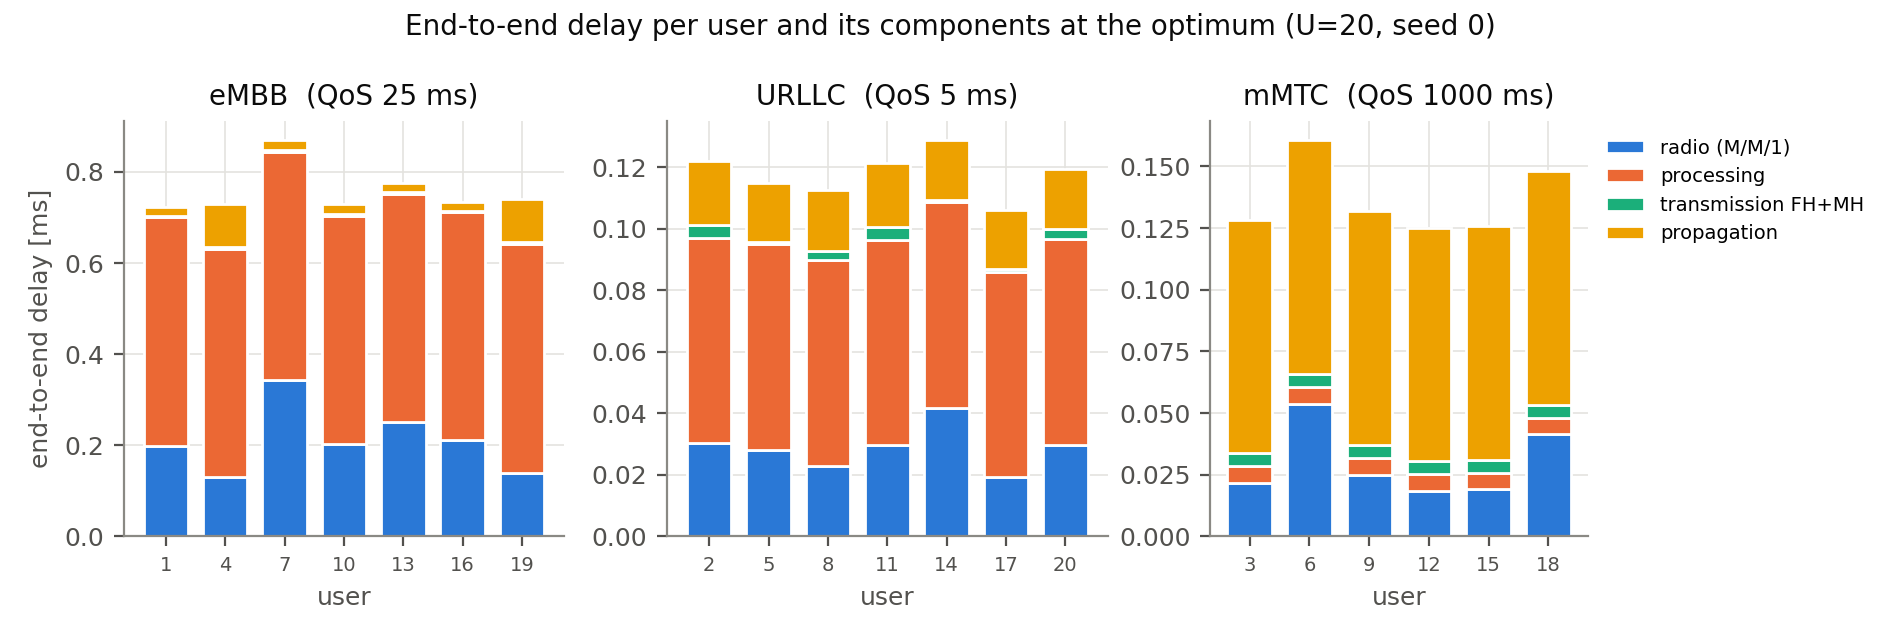
\includegraphics[width=\textwidth]{figures/system_delay.png}
	\caption{تأخیر انتها به انتهای هر کاربر و اجزای آن در جواب بهینه}\label{fig:delay}
\end{figure}

\paragraph{توان پردازشی.}
در شکل \ref{fig:proc} جواب بهینه بار را بین دو گره منطقه‌ای تقسیم می‌کند و بیشینه‌ی بهره‌وری پردازنده را از $3.7$ به $2.7$ درصد کاهش داده و صف پردازشی را کوتاه‌تر می‌کند. بهره‌وری پایین نشان می‌دهد که گلوگاه، ظرفیت منطقه‌ای نیست بلکه زمان سرویس هر بسته و هزینه‌ی گره‌های لبه است.

\begin{figure}[H]
	\centering
	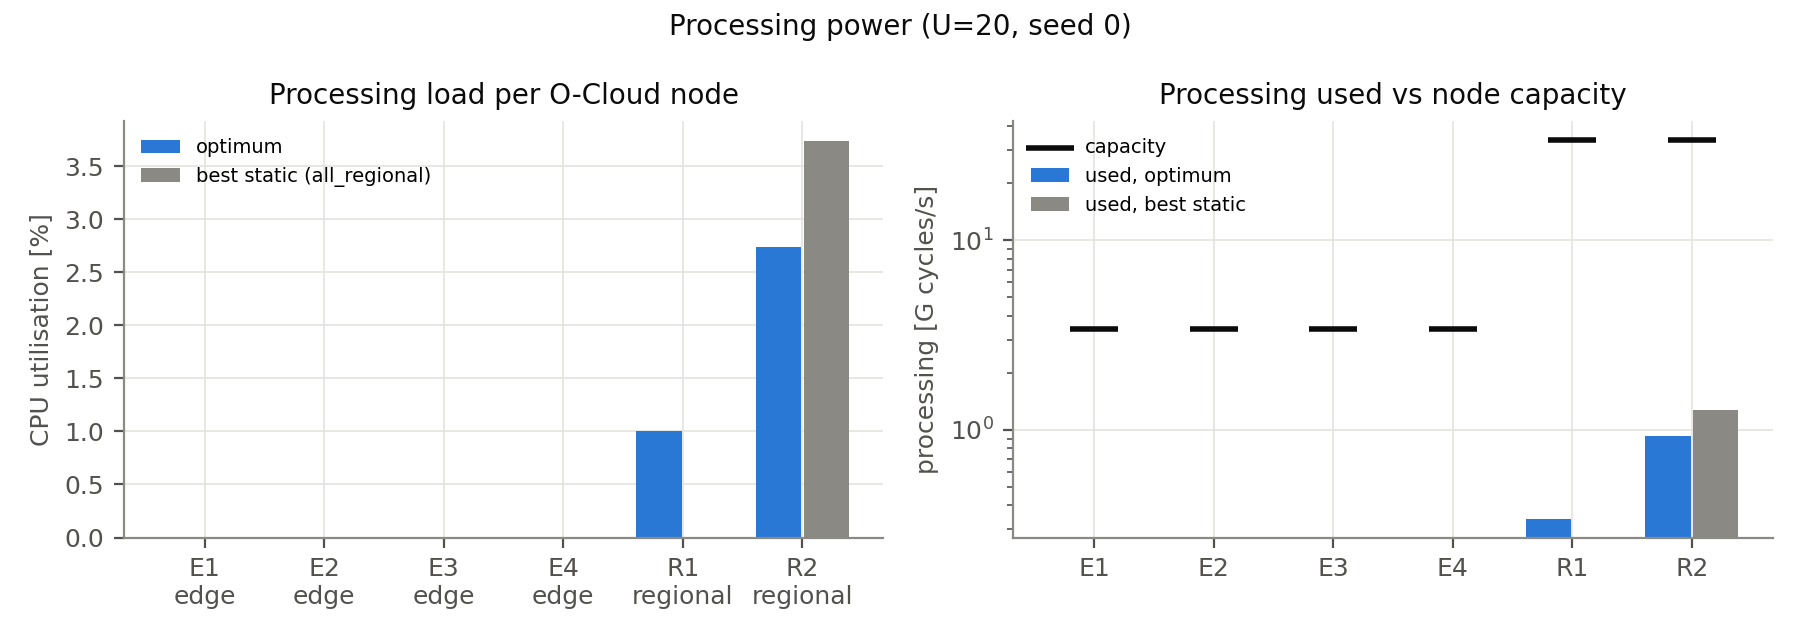
\includegraphics[width=\textwidth]{figures/system_processing.png}
	\caption{بهره‌وری و توان پردازشی مصرفی هر گره \lr{O-Cloud} در برابر ظرفیت آن}\label{fig:proc}
\end{figure}

\paragraph{واکنش برش‌ها.}
شکل \ref{fig:slices} واکنش هر برش به افزایش بار را نشان می‌دهد:
\begin{itemize}
	\item \textbf{\lr{eMBB} و \lr{URLLC}:} تأخیر در هر دو روش با بار افزایش می‌یابد، اما جواب بهینه تأخیر \lr{URLLC} را ۲۸ تا ۴۱ درصد کمتر نگه می‌دارد.
	\item \textbf{\lr{mMTC}:} برای $U\ge10$ تأخیر آن در جواب بهینه کمی بیشتر است ($0.09$ در برابر $0.065$ میلی‌ثانیه برای $U=20$). این نتیجه‌ی مستقیم وزن پایین آن ($\delta=0.1$) است: بهینه‌ساز منابع را به برش‌های حساس به تأخیر منتقل می‌کند.
	\item \textbf{نرخ:} نرخ دریافتی هر برش چندین برابر بار ارائه‌شده است؛ پس همه‌ی صف‌های رادیویی پایدارند و \lr{QoS} صد درصد کاربران برآورده می‌شود.
\end{itemize}

\begin{figure}[H]
	\centering
	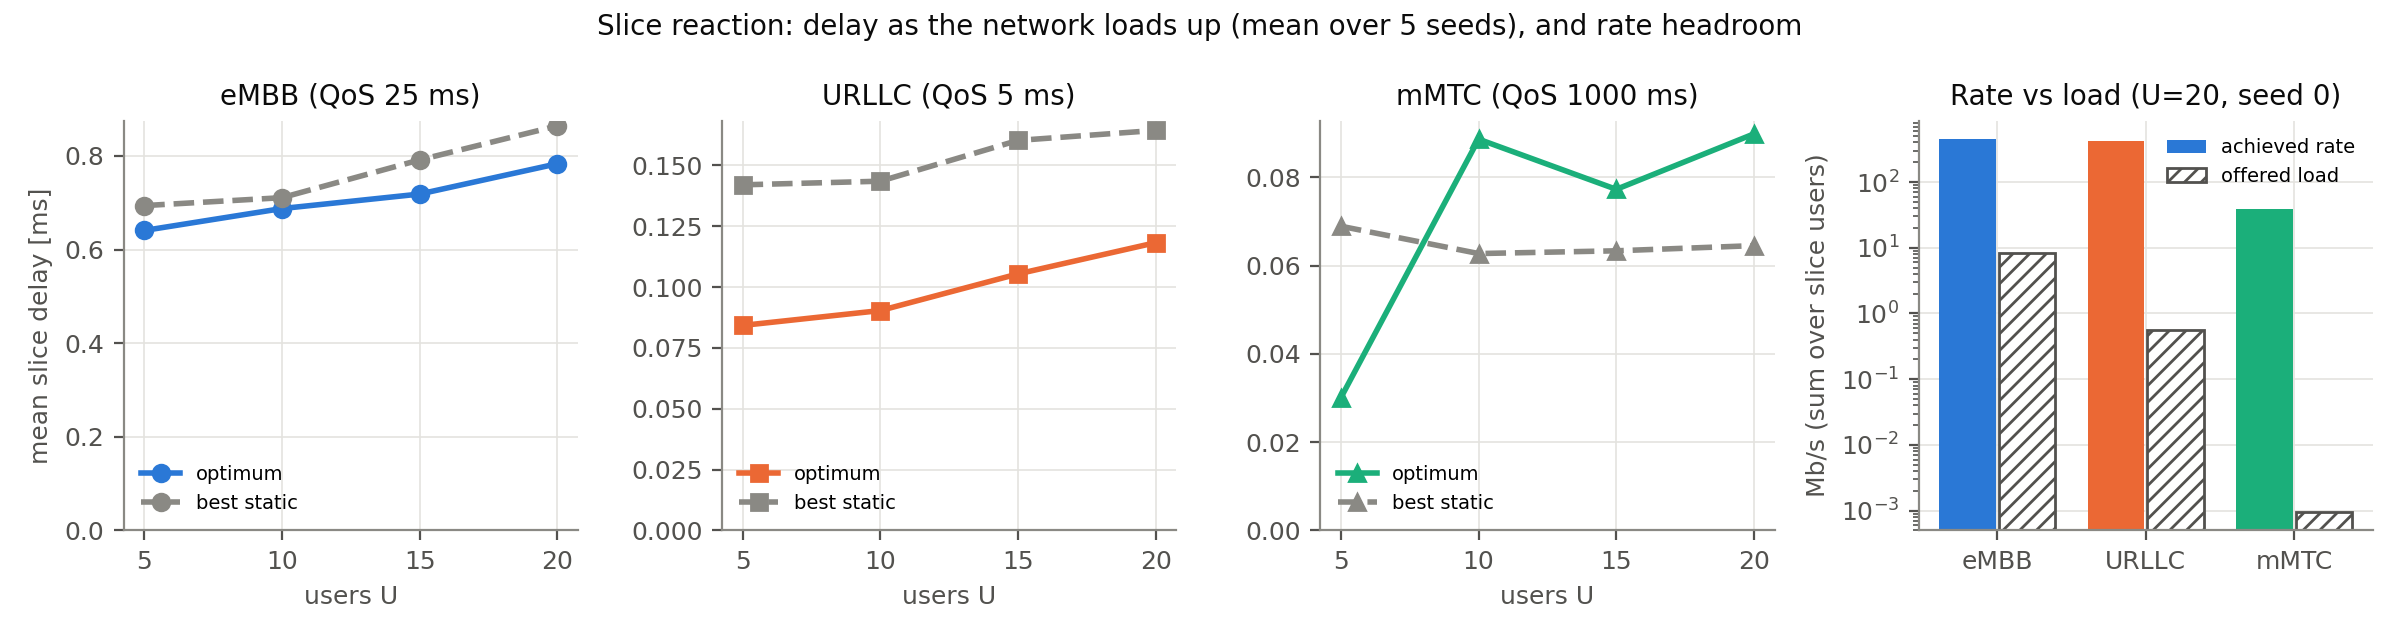
\includegraphics[width=\textwidth]{figures/system_slices.png}
	\caption{تأخیر میانگین هر برش بر حسب تعداد کاربران (جواب بهینه و بهترین ثابت) و نرخ دریافتی در برابر بار ارائه‌شده}\label{fig:slices}
\end{figure}

% =====================================================================================
\section{نتایج: یادگیری تقویتی}\label{sec:res_rl}
% TODO: با نتایج اجرای کامل (۴ روش × U∈{5,10,15,20} × ۳ seed × ۱۰۰۰ اپیزود) جایگزین شود.
این نتایج \textbf{مقدماتی} هستند: یک اجرای آزمایشی با $U=5$ و ۱۵۰ اپیزود، روی نمونه‌ای که جواب بهینه‌ی آن معلوم است. معیار، فاصله‌ی سیاست آموخته‌شده (بدون کاوش) از جواب بهینه است.

\begin{table}[H]
	\centering
	\caption{بهترین سیاست آموخته‌شده در برابر جواب بهینه (اجرای آزمایشی، $U=5$، ۱۵۰ اپیزود)}\label{tab:rl_pilot}
	\begin{latin}
		\begin{tabular}{lccc}
			\toprule
			Method & without prior & with residual prior & $J$ (with prior) \\
			\midrule
			TD3 + convex          & +12.4\% & \textbf{+2.2\%} & 0.0308 \\
			SAC + convex          & +26.2\% & +5.9\%  & 0.0319 \\
			MARL (2$\times$TD3)   & +54.2\% & +7.2\%  & 0.0323 \\
			single SAC            & +150\%  & +12.0\% & 0.0337 \\
			\midrule
			best static           & \multicolumn{2}{c}{+13.2\%} & 0.0341 \\
			optimum               & \multicolumn{2}{c}{0}       & 0.0301 \\
			\bottomrule
		\end{tabular}
	\end{latin}
\end{table}

\begin{figure}[H]
	\centering
	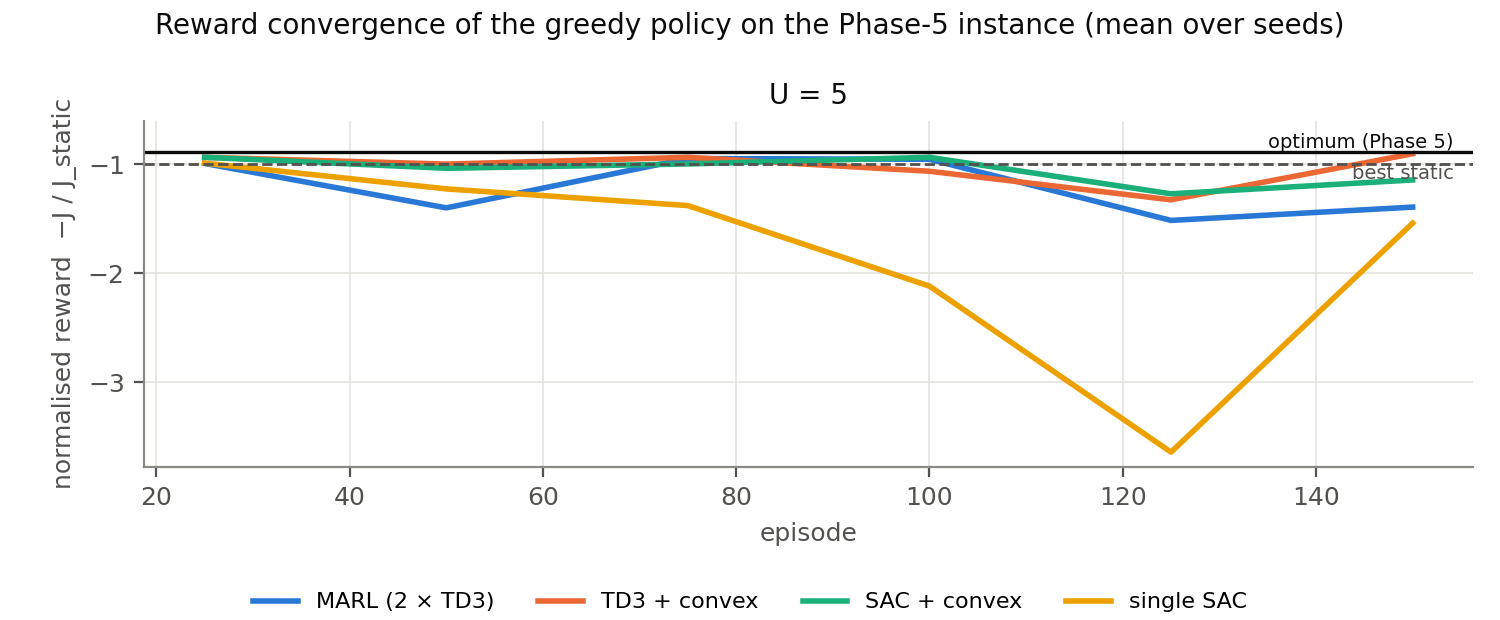
\includegraphics[width=0.75\textwidth]{figures/rl_reward_convergence.png}
	\caption{پاداش نرمال‌شده‌ی $-J/J_{\text{static}}$ سیاست آموخته‌شده روی نمونه‌ی مرجع؛ خط پر: جواب بهینه، خط‌چین: بهترین سناریوی ثابت (اجرای آزمایشی، $U=5$)}\label{fig:rl}
\end{figure}

\begin{itemize}
	\item \textbf{پیشین باقیمانده ضروری است}: با آن هر چهار روش از بهترین سناریوی ثابت بهترند. بدون آن، عامل بزرگ که در هر اپیزود فقط ۱۰ انتقال دریافت می‌کند، بیشتر آموزش را صرف یافتن یک پیکربندی قابل قبول از نقطه‌ی تصادفی می‌کند.
	\item \textbf{روش \lr{TD3} + بهینه‌سازی محدب به جواب بهینه نزدیک‌تر است} (۲.۲ درصد): بخش پرتکرار و پیوسته (بلوک و توان) دقیق حل می‌شود و عامل فقط تصمیم‌های گسسته‌ی کم‌تکرار را یاد می‌گیرد.
	\item \textbf{\lr{MARL} و \lr{SAC} واحد که بلوک و توان را نیز یاد می‌گیرند}، فاصله‌ی بیشتر و ناپایداری بیشتری دارند. در $U\ge10$ این عامل‌ها به سمت عمل‌های اشباع‌شده می‌روند که منابع را روی چند کاربر متمرکز کرده و \lr{QoS} و پایداری صف را نقض می‌کنند؛ ضریب $\tau=1$ و جریمه‌ی $c_a$ در \eqref{eq:reward} برای مقابله با آن به کار رفته‌اند. % TODO: تنظیم نهایی تأیید شود
	\item \textbf{زمان تصمیم‌گیری:} یک گذر رو به جلو \lr{actor} (لایه‌های ۱۰۲۴ و ۵۱۲) برای $U=20$ حدود $2.5$ میلی‌ثانیه روی یک هسته‌ی پردازنده طول می‌کشد، در حالی که بهینه‌سازی برای $U=10$ حدود ۴۷ دقیقه زمان می‌برد.
\end{itemize}

% =====================================================================================
\section{جمع‌بندی}\label{sec:summary}
\begin{itemize}
	\item بهینه‌سازی مشترک اتصال، بلوک، توان و جاگذاری \lr{CU}/\lr{DU} تابع هدف را ۱۸ تا ۳۳ درصد نسبت به بهترین سناریوی ثابت کاهش می‌دهد. این نتیجه با یک کران پایین تضمین‌شده پشتیبانی می‌شود (فاصله‌ی شرطی کمتر از $1.5$ درصد).
	\item جاگذاری در ابر منطقه‌ای با افزایش بار سودمندتر می‌شود (سهم لبه از ۶۵ به ۳۵ درصد). جداسازی \lr{CU} و \lr{DU} فقط در بار بالا و برای بخشی از واحدها انتخاب می‌شود، زیرا تأخیر \lr{midhaul} و قید زمان‌بندی را اضافه می‌کند.
	\item بهینه‌ساز بر اساس وزن برش‌ها منابع را از \lr{mMTC} به \lr{URLLC} و \lr{eMBB} منتقل کرده و تأخیر \lr{URLLC} را ۲۸ تا ۴۱ درصد کاهش می‌دهد.
	\item در میان روش‌های یادگیری تقویتی، ترکیب یک عامل مقیاس بزرگ با بهینه‌سازی محدب در مقیاس کوچک به جواب بهینه نزدیک‌تر است و برای اجرای برخط به اندازه‌ی کافی سریع است. % TODO: با نتایج کامل تأیید شود
\end{itemize}

\end{document}
